\begin{section}{Results}
 The algorithm was tested with some provided instances, whose parameters are shown in Table \ref{tab:parameters} along with
 the chose size for the tabu list.
 In all the instances, the algorithm was able to reach a solution where no hard constraint was violated,
 with penalty values shown in Table \ref{tab:penalties}.


 \begin{table}[h]
     \centering
     \begin{tabular}{lllllllll}
         \hline
         \textbf{Instance} & \textbf{Days} & \textbf{Shifts} & \textbf{Occupants} & \textbf{Patients} & \textbf{\begin{tabular}[c]{@{}l@{}}Operating\\ Theaters\end{tabular}} & \textbf{Rooms} & \textbf{Nurses} & \textbf{Tabu List Size} \\ \hline
         toy               & $7$           & $3$             & $2$                & $7$               & $1$                                                                   & $3$            & $11$            & $30$                    \\
         $1$               & $21$          & $3$             & $7$                & $42$              & $2$                                                                   & $5$            & $13$            & $150$                   \\
         $2$               & $14$          & $3$             & $5$                & $37$              & $4$                                                                   & $6$            & $17$            & $200$                   \\
         $3$               & $14$          & $3$             & $10$               & $45$              & $2$                                                                   & $6$            & $14$            & $200$                   \\
         $4$               & $14$          & $3$             & $7$                & $54$              & $3$                                                                   & $8$            & $19$            & $250$                   \\
         $6$               & $14$          & $3$             & $8$                & $110$             & $3$                                                                   & $9$            & $20$            & $1$                     \\
     \end{tabular}
     \caption{Test instances parameters and tabu list size.}
     \label{tab:parameters}
 \end{table}
 \begin{table}[h]
     \centering
     \begin{tabular}{llll}
         \hline
         \textbf{Test Instance} & \textbf{Starting penalty} & \textbf{Tabu Penalty} & \textbf{Proposed Penalty} \\ \hline
         toy                    & $0$                       & $269$                 & $292$                     \\
         $1$                    & $0$                       & $3976$                & $3177$                    \\
         $2$                    & $0$                       & $2443$                & $1583$                    \\
         $3$                    & $0$                       & $11624$               & $10184$                   \\
         $4$                    & $0$                       & $6524$                & $2332$                    \\
         $6$                    & $0$                       & $25366$               & $17048$                   \\
     \end{tabular}
     \caption{Penalty reached by the Tabu Search algorithm on the test instances, compared to the
         penalties of the starting configuration and the competition proposed solution.}
     \label{tab:penalties}
 \end{table}

 \begin{figure}
     \centering
     \begin{subfigure}{0.45\textwidth}
         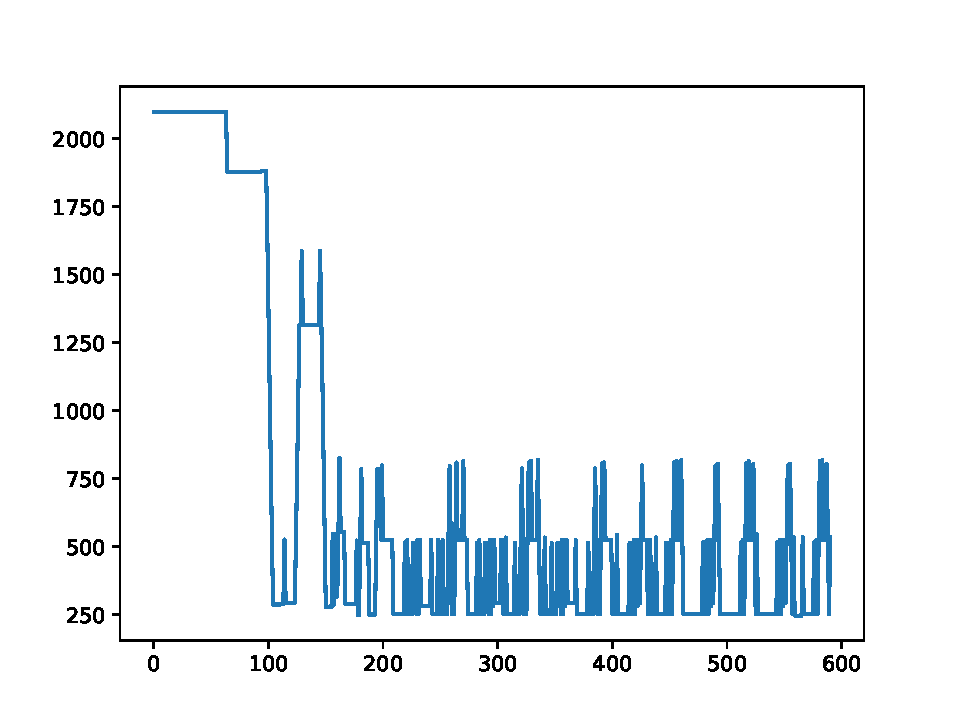
\includegraphics[width=\textwidth]{../logs/toy.pdf}
         \caption{Toy.}
     \end{subfigure}
     \begin{subfigure}{0.45\textwidth}
         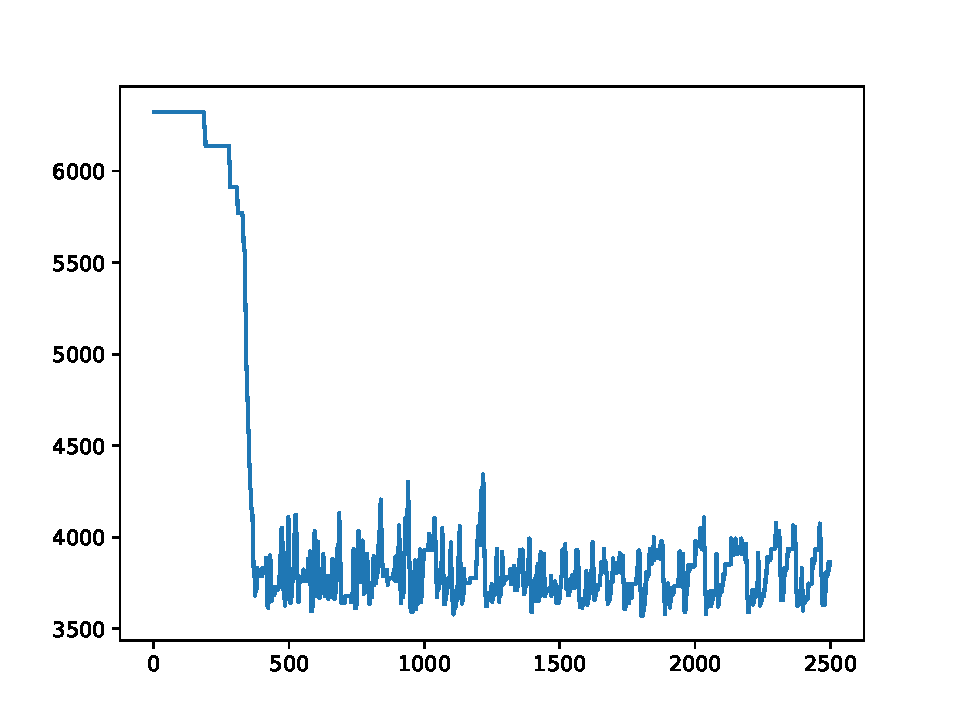
\includegraphics[width=\textwidth]{../logs/test01.pdf}
         \caption{Test $01$.}
     \end{subfigure}
     \begin{subfigure}{0.45\textwidth}
         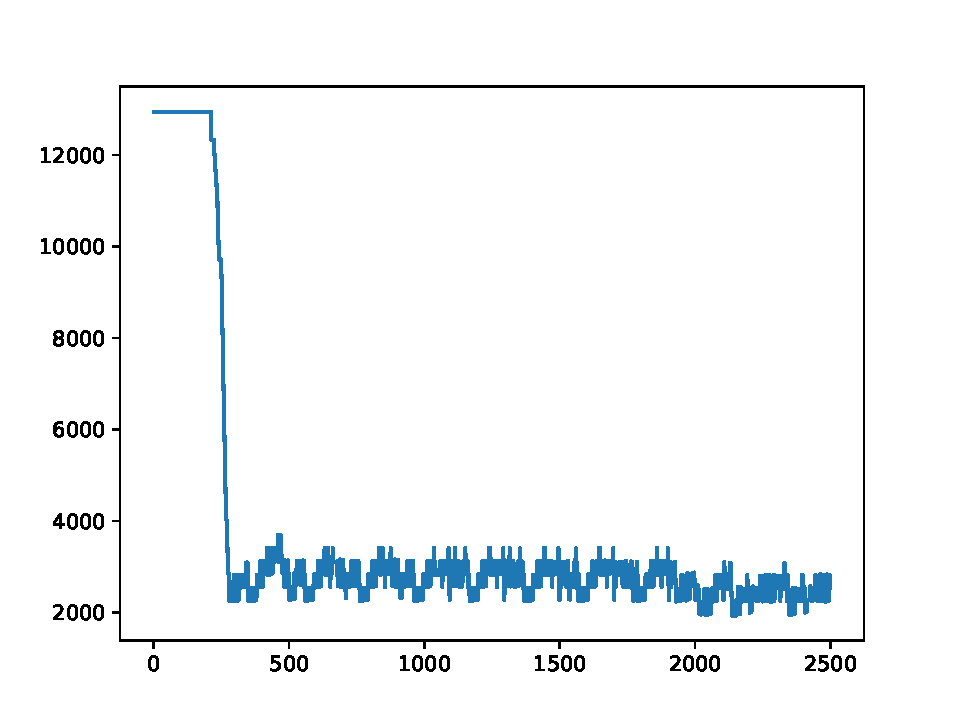
\includegraphics[width=\textwidth]{../logs/test02.pdf}
         \caption{Test $02$.}
     \end{subfigure}
     \begin{subfigure}{0.45\textwidth}
         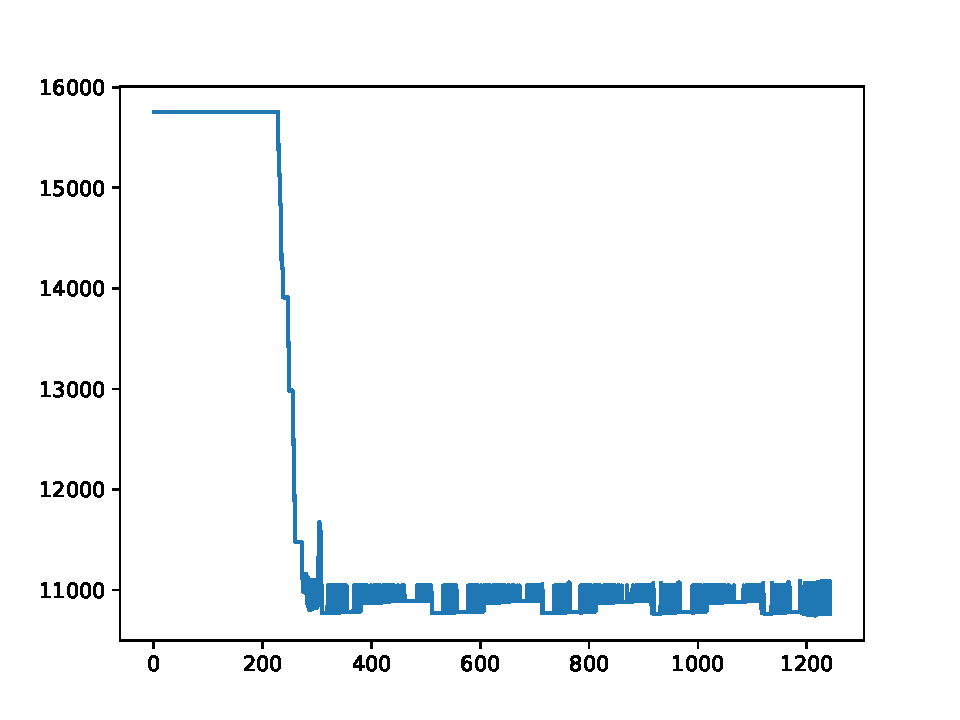
\includegraphics[width=\textwidth]{../logs/test03.pdf}
         \caption{Test $03$.}
     \end{subfigure}
     \begin{subfigure}{0.45\textwidth}
         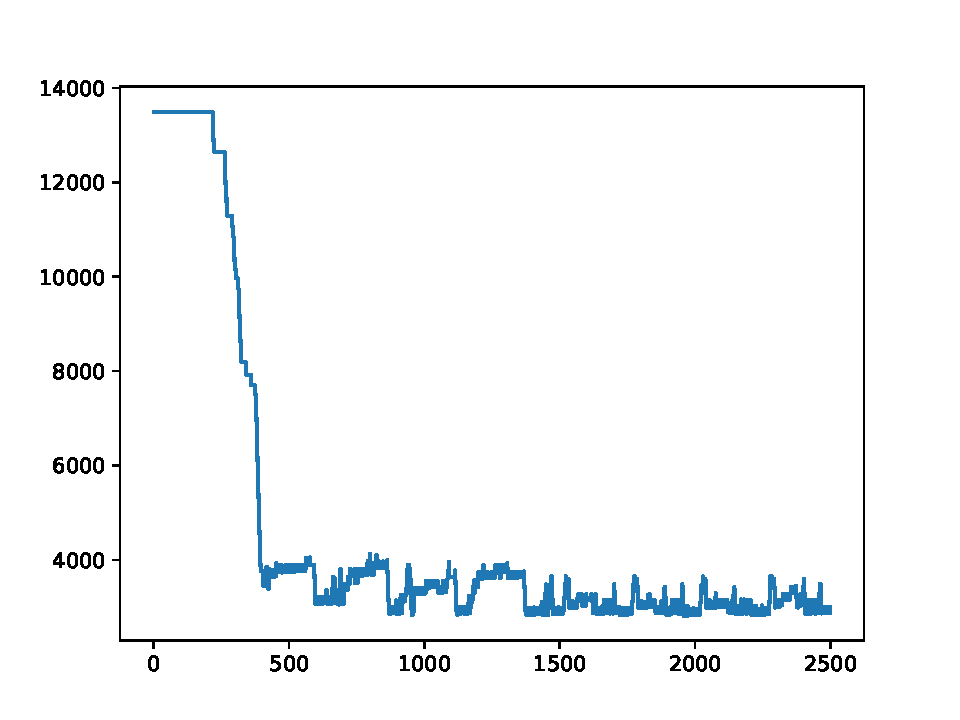
\includegraphics[width=\textwidth]{../logs/test04.pdf}
         \caption{Test $04$.}
     \end{subfigure}
     \begin{subfigure}{0.45\textwidth}
         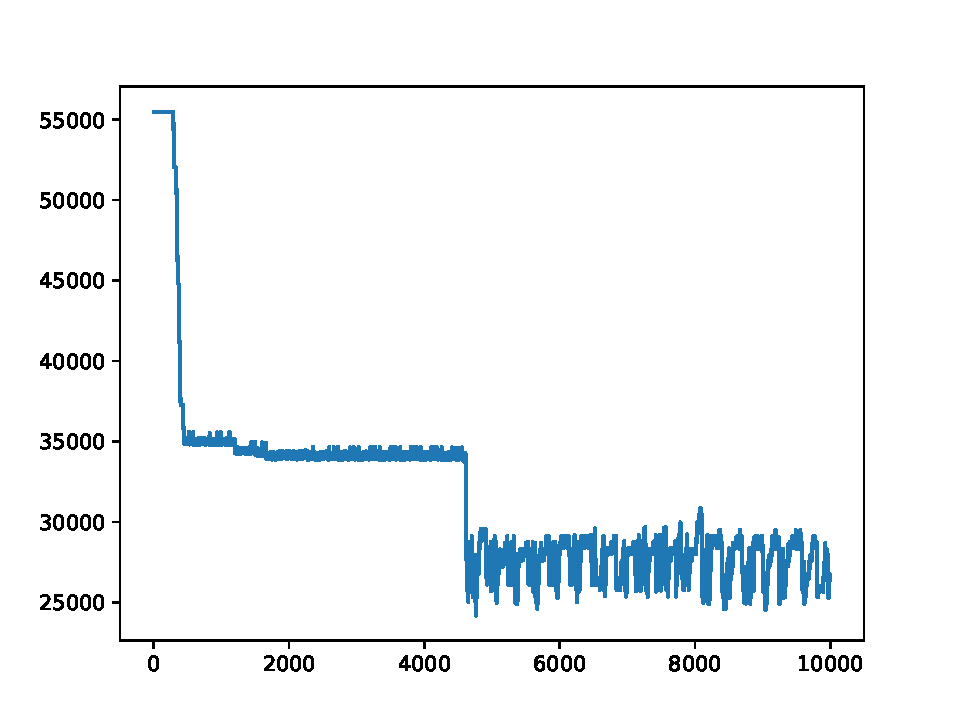
\includegraphics[width=\textwidth]{../logs/test06.pdf}
         \caption{Test $06$.}
     \end{subfigure}
     \caption{Costs of the solution found by the Tabu Search algorithm on the test instances.}
     \label{fig:plot}
 \end{figure}

\end{section}